% !TeX root = proposal.tex
\section{vTask}
\label{sec:vTask}

Specialized compute accelerators (e.g., TPUs, GPUs, IPUs) are rapidly proliferating in the data center. This trend is fueled by the emergence of workloads with an appetite for massive amounts of both data and compute, at a time when transistor shrinkage (Moore’s law) has slowed down and the Dark Silicon problem looms large. Hyperscalers are even deploying custom silicon in their data centers, e.g., Google Cloud TPUs, Amazon Nitro.

API-remoting based virtualization has been shown~\cite{trillium,ava-hotos}
to be the only effective mechanism for sharing these specialized compute devices among mutually distrustful tenants, e.g., in a cloud computing environment. Virtualization vendors, such as VMware, have begun adopting API-remoting based solutions for accelerator virtualization [cite BitFusion acquisition].

API-remoting works by interposing on API calls invoked by the application in the guest OS, and executing them in a surrogate, the executor, in the host. Typically, executors are associated with a single API framework (for modularity and failure isolation between APIs/accelerators) and each executor is a surrogate for a single guest (to preserve memory isolation between guests). Applications that use multiple accelerator API frameworks will be associated with multiple executors, one per framework.

\begin{figure}[ht!]
\centering
\captionsetup{justification=centering,width=\linewidth}
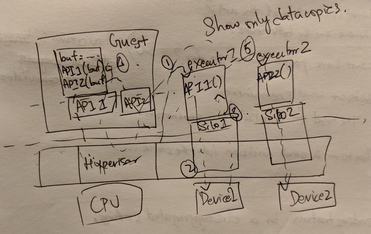
\includegraphics[width=0.5\linewidth]{figures/overview.png}
\caption{Data processed by two API stacks must pass through the guest application}
\label{fig:overview}
\end{figure}

Under a typical API-remoting system, applications that pipeline disparate accelerator frameworks are burdened with redundant data movement. All inter-accelerator data movement must take place in the guest application as that is where the accelerators are in the same logical address space. Figure~\ref{fig:overview} illustrates this scenario: when an API-1 function is invoked, associated data is copied from the guest application to executor-1, and then to device-1’s memory. Once the function finishes executing on device-1, the result is copied back to the guest VM. When a function from API-2 is invoked, the same data (i.e., the output of the API-1 function) is copied to executor-2 and then to device-2 to be processed.

In order to eliminate redundant data movement when an application uses multiple accelerators via API-remoting, the hypervisor must track the data passed to these API calls. The hypervisor must keep track of where the data flowed from and to, the validity of different copies of the data (e.g., if the data is modified on the accelerator, but hasn’t been copied back to the accelerator silo, or the guest application), and eliminate redundant data movement. As an example, if a guest application were to invoke the cudaMempyDtoH() function to copy data back from an Nvidia GPU, and then invoke the Intel QAT compression function cpaDCCompressData2() on the same data without modifying it in any way, the hypervisor should be able to detect this and elide the copying of data to and from the guest application.

vTask is an application-transparent data orchestration system that optimizes data movement among accelerators virtualized via API-remoting. vTask leverages information from API annotations (cite AvA) to track data buffers across the guest application, the executors servicing API calls made by the guest, and the accelerator hardware. vTask optimizes data movement across these components while ensuring that a coherent view of the data buffer is presented to anyone attempting to read the data. vTask requires no changes to the guest application or annotations of any kind from the application programmer; annotations provided to virtualize the API (by the device or virtualization vendor) are leveraged to infer semantics of the data buffers managed.

We prototyped vTask in AvA, a state-of-the-art para-virtual API-remoting system for KVM. vTask relies on device-side buffer allocation and deallocation API calls to determine buffer lifetime. vTask also leverages special annotations to explicitly specify buffer lifetime provided by LAPIS, AvA’s API description language. vTask implements a simple MESI-style coherence protocol to track spatial validity of data (i.e., to track where the latest data is present). vTask relies on optimizations such as shared memory, Unified Virtual Memory, and PCIe Peer-to-Peer (P2P) data transfer where available, but does not make assumptions about their universal availability.

vTask can handle data movement between both local and remote devices. When API-remoting to a remote system, the devices used by the guest application may be present on separate machines. vTask takes care to eliminate costly data transfers over the network by adhering to the principle of lazy loading wherever possible, i.e., data is not moved until a demand fault occurs.

Evaluating vTask on Y applications that different combinations of the ten accelerators supported by AvA shows that vTask improves performance by X\% on average when all devices are on the same machine, and Z\% when the devices are on remote hosts.

This work makes the following contributions:
\begin{itemize}[nosep,leftmargin=1em,labelwidth=*,align=left]
\item We identify and measure performance problems with using multiple accelerators via API-remoting
\item We propose an application-transparent data orchestration framework, vTask, which transparently manages data buffers in the hypervisor and elides redundant data movement.
\item We prototyped vTask in AvA with support for both local and remote accelerators, and used it to evaluate the performance of applications that use different combinations of the ten accelerators supported by AvA. vTask improves application performance by XX% on average.
\end{itemize}